\section{TP4 Separate user identity, sign-up and self-care from product dependencies}
\label{sec:principle-tp4-seperate-user-identity}

Viele Dienste im Internet verlangen heute die Erstellung eines Benutzerkontos. Ein Forum lässt bspw. das Verfassen von Beiträgen erst zu, nachdem sich der potentielle Autor mit seiner E-Mail-Adresse, einem Benutzernamen und einem Passwort erfolgreich registriert hat. Zur Praxis gehört zudem, dass der Benutzer seine Angaben mittels einem eindeutigen Link, welcher ihm per E-Mail zugestellt wird, bestätigt.

Eine solche Registrierung hat sowohl für den Benutzer eines Dienstes als auch für den Betreiber dessen auf den ersten Blick hauptsächlich Vorteile:

\begin{itemize}
	\item Die User Experience kann von Anfang bis Ende auf den Benutzer zugeschnitten und optimiert werden. (Beispiele: Speichern der eigenen Zeitzone für korrekte Termin- und Zeitangaben, Personalisierung der Frontseite usw.)
	\item Sicherstellung der Identität: Jedes Benutzerkonto resp. jeder Benutzername wird immer von derselben Person verwendet
	\item Durch gezielte Auswertungen kann der Betreiber sein Angebot optimieren und ggf. Marketing betreiben resp. Werbung in seinem Dienst schalten
\end{itemize}

Bei genauerer Analyse ergeben sich aber auch nicht zu vernachlässigende negative Faktoren:

\begin{itemize}
	\item Der Benutzer muss bei jedem neuen Dienst wiederholt ein Konto erstellen und so erneut persönliche Informationen preisgeben
	\item Der Betreiber muss sich um die Speicherung und Sicherheit der Benutzerinformationen kümmern
	\item Der Mechanismus zur Identitätsüberprüfung muss vom Betreiber selbst umgesetzt werden
	\item Nach einer gewissen Zeit hat ein Benutzer tendenziell keine Kontrolle mehr darüber, wo er sich registriert und seine Informationen hinterlegt hat
	\item Die Umsetzung von Zugriffskontrollen (Wer darf welche Informationen eines Benutzers sehen etc.) ist mit entsprechendem Aufwand verbunden
\end{itemize}

Tilkovs \emph{TP4} schlägt nun die generelle Separierung von Benutzerinformationen und der eigentlichen Registrierung bei einem Dienst vor.

Der Vorreiter OpenID \cite{OpenID} und insbesondere die omnipräsenten sozialen Netzwerke erleichtern resp. forcieren eben diese Auftrennung heute mehr den je.
\newline\newline
Ein Konto bei Facebook oder Twitter ermöglicht so den Zugriff auf Dienste Dritter: Möchte ein Benutzer personalisierte News bei \emph{20 Minuten} lesen, kann er sich mit seinem Facebook Konto anmelden \cite{20min} ohne genauere Informationen zu seiner Person wiederholt angeben zu müssen. Dabei kann er zudem gezielt steuern, welche Informationen an den Dienstbetreiber durch Facebook weitergegeben werden und welche nicht.

\begin{figure}[H]
	\centering
	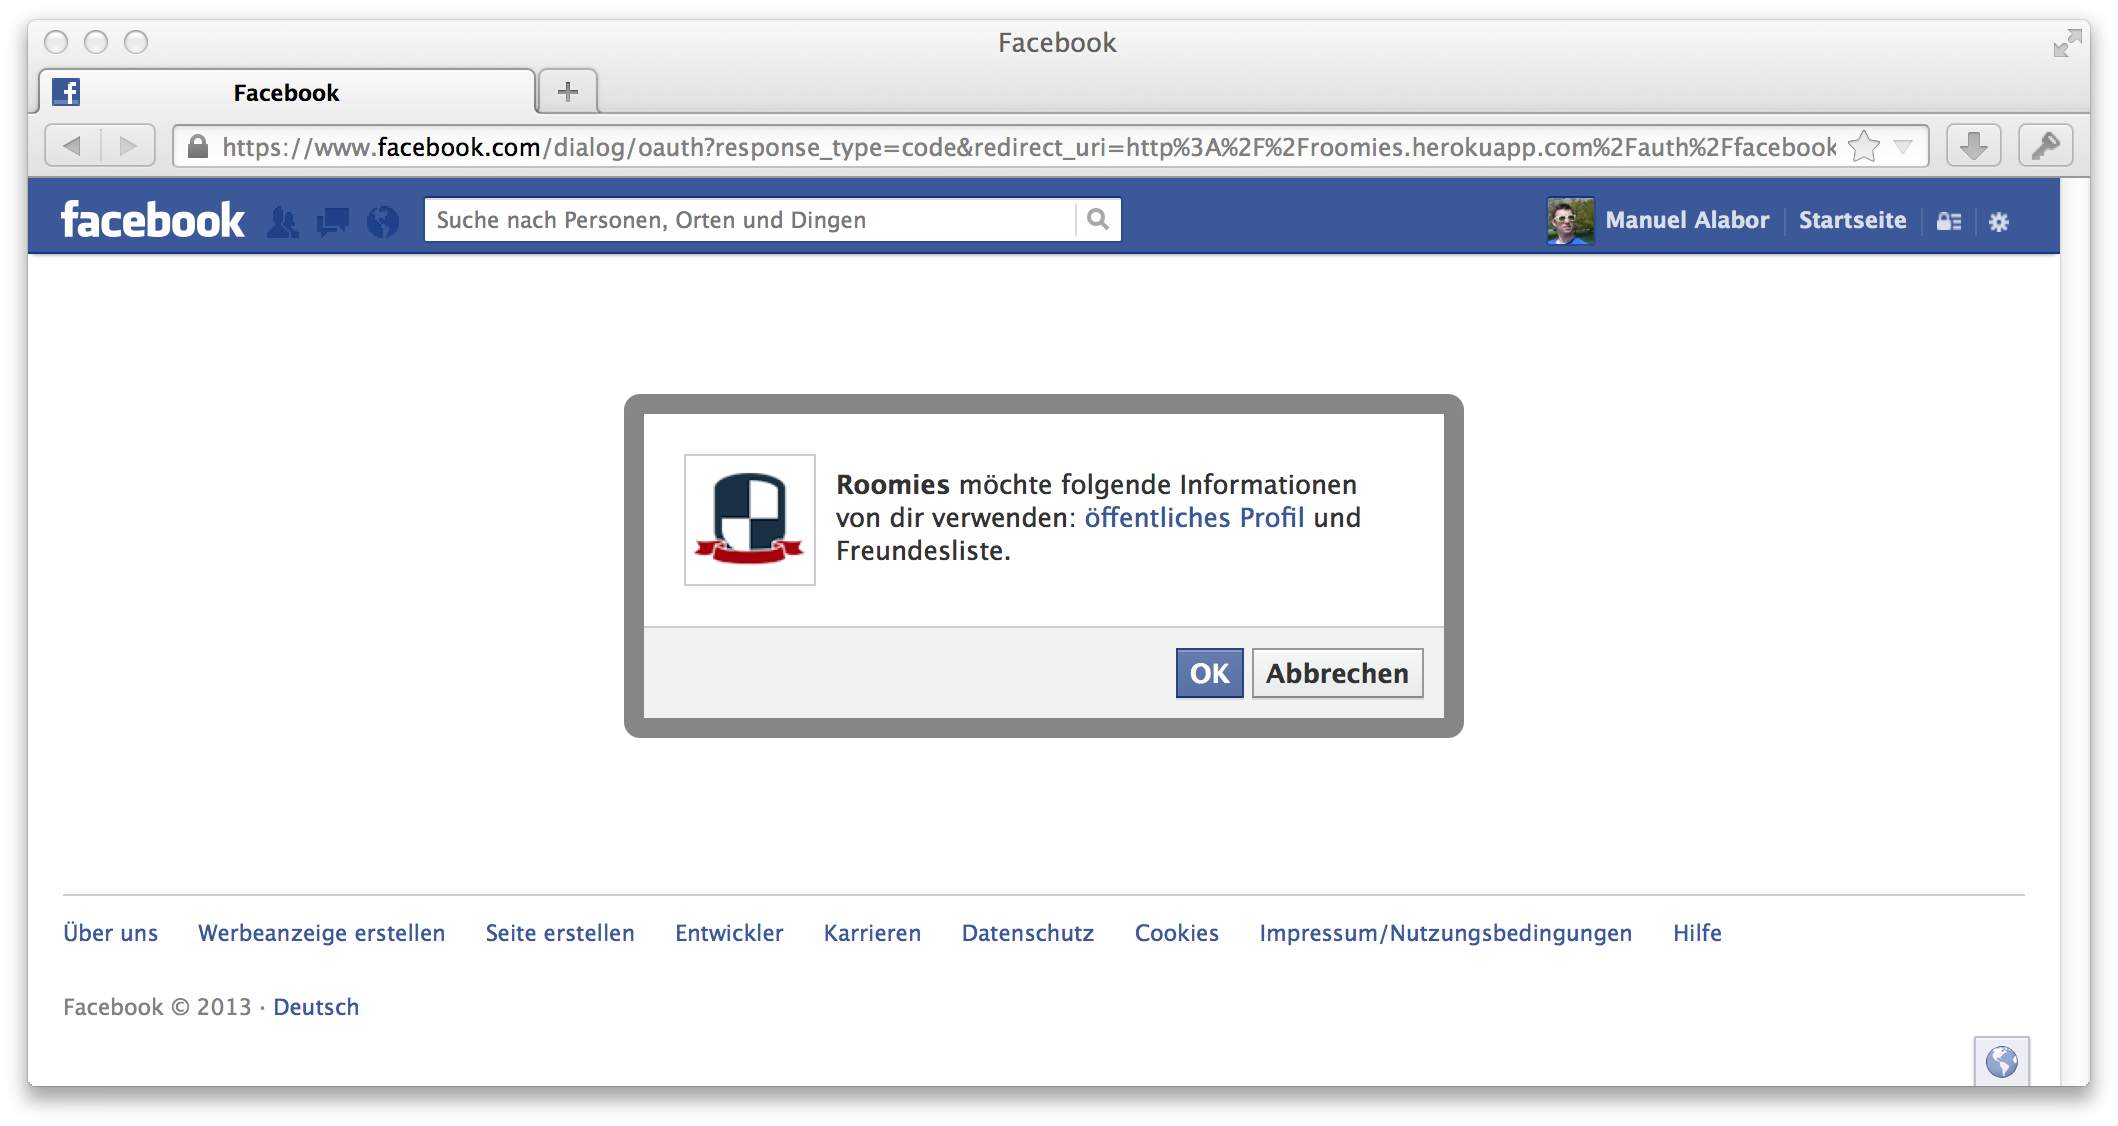
\includegraphics[width=10cm]{content/principle-demonstration/images/facebook-auth-dialog.png}
	\caption{Bestätigungsdialog von Facebook, ob \emph{Roomies} auf die persönlichen Daten des Benutzers zugreifen darf.}
	\label{fig:facebook-auth-dialog}
\end{figure}


Visualisiert sieht das Konzept der getrennten Datenhaltung in Bezug auf applikations- und identitätsspezifsche Informationen wie in Abbildung \ref{fig:applicationdata-vs-identityprovider} aus.

\begin{figure}[H]
	\centering
	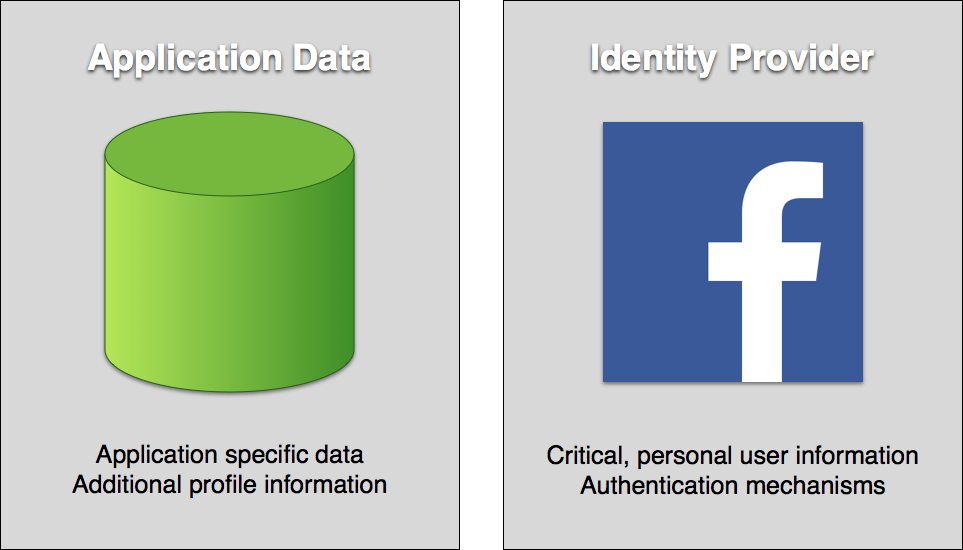
\includegraphics[width=9cm]{content/principle-demonstration/images/applicationdata-vs-identityprovider.png}
	\caption{Separierung der Applikations- und Identitätsinformationen}
	\label{fig:applicationdata-vs-identityprovider}
\end{figure}

Zudem ist in Abbildung \ref{fig:applicationdata-vs-identityprovider} ersichtlich, dass ein \emph{Identity Provider} meist auch den Mechanismus zur effektiven Authentisierung des Benutzers bereitstellt. Viele Anbieter setzen hier auf den de facto Standard \emph{OAuth} \cite{oauth} oder verwenden eigene Implementationen.


\subsection*{Geplante Umsetzung}

Für die Beispielapplikation \emph{Roomies} hat das Projektteam geplant, Facebook als hauptsächlichen und einzigen \emph{Identity Provider} einzusetzen. Dabei soll das offizielle \emph{Facebook Login for Web} \cite{facebooklogin} \gls{SDK} eingesetzt werden.

Innerhalb der Beispielapplikation soll lediglich die Facebook ID sowie der Name des Benutzers persistent gespeichert werden. Alle anderen Informationen sollen bei Facebook verbleiben.


\subsection*{Konkrete Umsetzung}

Die tatsächliche Anbindung des ``\emph{Facebook Login for Web}'' \cite{facebooklogin} \gls{SDK}'s wurde wie in Abschnitt \ref{sec:sad-layers} ``\nameref{sec:sad-layers}'' des Kapitels ``\nameref{sec:sad}'' beschrieben, mithilfe der quelloffenen Bibliothek \emph{Passport.js} \cite{Passportjs} umgesetzt.

Die verfügbare \emph{Authentication Strategy} für Facebook \cite{passport-facebook} ermöglicht das einfache Einbinden der Facebook Anmeldemechanismen in jede \emph{Express.js} Applikation.

Zudem werden wie geplant lediglich Facebook ID und der Name des Benutzers in der Applikationsdatenbank abgelegt. Über eine öffentlich zugängliche \gls{URL} \cite{facebook-profilepicture} wird zusätzlich das aktuelle Profilbild des Benutzers in der Menüleiste von \emph{Roomies} angezeigt, jedoch nicht innerhalb der Applikation zwischengespeichert.

\begin{figure}[H]
	\centering
	
\includegraphics[width=10cm]{content/principle-demonstration/images/roomies-navigation-loggedin.png}
	\caption{Facebook Profilbild des angemeldeten Benutzers der Menüleiste der Beispielapplikation \emph{Roomies}}
	\label{fig:facebook-profilepicture-roomies}
\end{figure}


\subsection*{Diskussion}

Lange Zeit hielten sich hartnäckige Vorbehalte gegenüber der Verwendung von Facebook oder ähnlichen Konten für die Anmeldung bei Diensten Dritter. Immer mehr lässt sich jedoch eine gewisse Akzeptanz bei den Benutzern im Internet feststellen. Verbesserte und klarer deklarierte Möglichkeiten zur Anpassung der Zugriffseinstellungen auf hinterlegte Informationen \cite{facebook-authdialog} haben hier definitiv ihren Teil beigetragen.

Für den Dienstanbieter bringt die Verwendung eines externen \emph{Identity Providers} grosse Vorteile mit sich: Er kann sich auf seine Kernkompetenzen konzentrieren, insbesondere wenn zur Integration umfangreiche Frameworks wie eben \emph{Passport.js} \cite{Passportjs} verwendet werden können.

So ist es ohne grössere Zusatzaufwände möglich (eine entsprechende Architektur vorausgesetzt) weitere \emph{Provider} anzubinden. Im Falle der vorliegenden Beispielapplikation ist die Integration von \emph{Twitter} (um nur einen \emph{Identity Provider} zu nennen) genau so einfach umsetzbar, wie die Implementation einer komplett eigenständigen Lösung.

Welche Möglichkeiten zur Anmeldung bei einem Dienst angeboten werden sollen ist -- wie so oft -- von verschiedensten Faktoren abhängig:

\begin{itemize}
	\item Datenschutz
	\item Potentielle Akzeptanz bei Benutzern
	\item Verbreitung spezifischer \emph{Identity Providers} bei Benutzern
	\item Usability \& User Experience
	\item Neue oder bestehende Applikation?
\end{itemize}

Gerade bei Applikationen aus einem tendenziell kritischen Geschäftsfeld wie eBanking-Suiten mag es heute lächerlich klingen, sich via Facebook-Konto anzumelden. Die grosse Verbreitung von PayPal \cite{paypal} als zentralen Anbieter von Geldtransaktionsdiensten zeigt aber, dass selbst hier mit entsprechenden Sicherheitsmassnahmen viel Skepsis erfolgreich wettgemacht werden kann.

Lassen es die Anforderungen einer Applikation zu, so empfiehlt das Projektteam zum heutigen Zeitpunkt die von \emph{TP4 Separate user identity, sign-up and self-care from product dependencies} vorgeschlagene Teilung von Applikations- und Identitätsinformationen resp. Authentifizierungsmechanismen.
